\chapter{Prototype} \label{ch:prototype}
The code for the prototype developed in this thesis is available at:\\
\url{https://github.com/flol3622/LDBIM-viewer}.

\section{Database design}
The database used in this thesis is based on the database developed by Mads Holten Rasmussen and made available at:\\
\url{https://github.com/MadsHolten/BOT-Duplex-house/tree/master/Model%20files/LBD}

It was chosen as a starting point, as it already contained \ac{bot} descriptions and relations between entities which are heavily utilized by this thesis' algorithm. Additionally, it was selected because it already contained geometry descriptions of those entities. As well as containing \ac{wkt} serializations of walls, rooms, and floor entities. Although the size of the model it describes is small, too small to evaluate culling performance, no other suitable database meeting the requirements was found.

Nevertheless, some changes had to be made to accommodate the needs of this thesis. This section will describe these changes.

\subsection{GraphDB}
To host the database, and exercise the role of the \ac{sparql} endpoint, a GraphDB instance was run locally to store, query, modify, and extract the semantic data. \enquote{GraphDB is an enterprise ready Semantic Graph Database, compliant with W3C Standards}\footcite{graphdb} It was chosen for its simple installationa and application, its support for the GeoSPARQL extension (Section \ref{sec:inSituWKT}), as well as the possibility to create custom functions in JavaScript (Section \ref{sec:inQuery}).

To comply with the requirements of the algorithm, the structure of the database had to be altered to resemble the one illustrated in Figure \ref{fig:omg1}. Figure \ref{fig:dbadaptation} illustrates the changes made to the database, where the existing data was used to describe new relations needed for this thesis.

\begin{figure}[H]
    \centering
    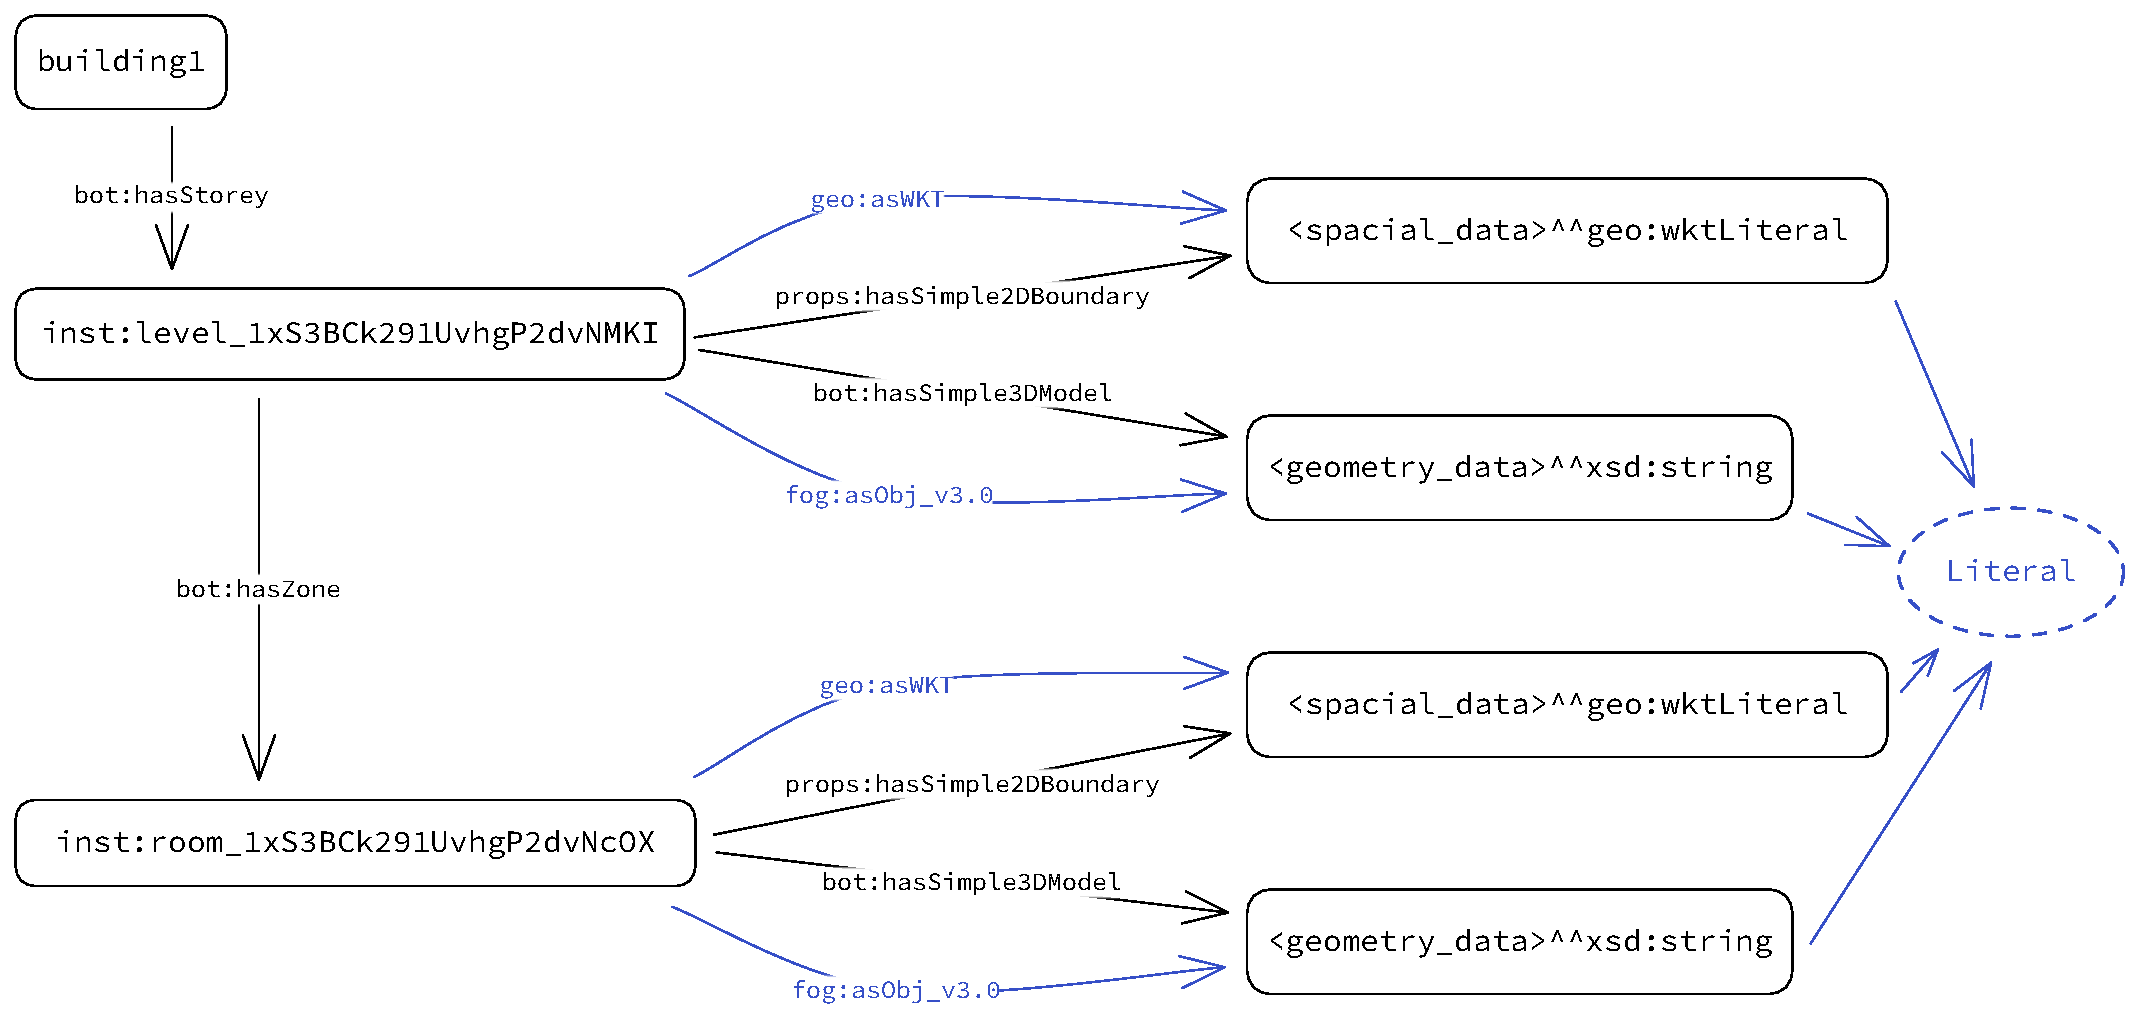
\includegraphics[width=\textwidth]{figures/pdf/dbadaptation.pdf}
    \caption[Database adaptation]{Database adaptation to Figure \ref{fig:omg1}.}
    \label{fig:dbadaptation}
\end{figure}

\subsection{3D geometries}
Listing \ref{lst:insertFOG} demonstrates how the \ac{fog} ontology was implemented in the \ac{rdf} database. The following subsections describe the additional steps taken to adapt the database to the specific requirements of the viewer used.

\begin{listing}[H]
    \begin{minted}{sparql}
PREFIX bot: <https://w3id.org/bot#>
PREFIX fog: <https://w3id.org/fog#>

INSERT { ?s fog:asObj_v3.0 ?o . }
WHERE { ?s bot:hasSimple3DModel ?o . }
    \end{minted}
    \caption[Inserting \acs{fog} relations]{Inserting \acs{fog} relations into the database.}
    \label{lst:insertFOG}
\end{listing}

\subsubsection{Extracting geometries from \ac{rdf} database}
Due to the inability to display OBJ literals in the utilized viewer, the geometries had to be extracted from the database and stored as separate files. This was accomplished using a Python script (Appendix \ref{sec:pyhtonExtraction}), which extracted the geometries from the database using Listing \ref{lst:extractGeometries} and stored them as separate files.

\begin{listing}[H]
    \begin{minted}{sparql}
SELECT ?s ?o
WHERE {
    SERVICE <http://localhost:7200/repositories/duplex-v1> {
        ?s fog:asObj ?o .
        filter(datatype(?o)=xsd:string)
    }
}
    \end{minted}
    \caption{\acs{sparql} query to extract geometries.}
    \label{lst:extractGeometries}
\end{listing}


\subsubsection{Rescaling geometries}
Rescaling the entities to fit the viewer's coordinate system was executed by using the open-source 3D modeling software, Blender. This software allowed for the batch import, rescale, and export of the different entities. However, batch export into multiple files was restricted to the STL file format only. After which, the individual files were uploaded to the \href{https://github.com/flol3622/LDBIM-viewer}{GitHub repository} of the prototype, which functioned as an external database.

\subsubsection{Inserting data}

The new external files were inserted in the database using the \ac{sparql} query in Listing \ref{lst:insertLinks}. This query designated the literal's datatype as \mintinline{turtle}|xsd:anyURI| (Section \ref{sec:fog}), which the prototype would later use to treat the resource as a link to an external file (Section \ref{sec:databaseFetcher}).

\begin{listing}[H]
    \begin{minted}{sparql}
PREFIX fog: <https://w3id.org/fog#>
PREFIX xsd: <http://www.w3.org/2001/XMLSchema#>

INSERT { ?s fog:asStl_v1.0-ascii ?newURI }
WHERE { 
    ?s fog:asObj_v3.0 ?o .
    FILTER (datatype(?o) = xsd:anyURI)
    BIND (REPLACE(STR(?s), "https://172.16.10.122:8080/projects/1001/", "") AS ?localName)
    BIND (REPLACE(STR(?localName), "%", "-") AS ?newLocalName)
    BIND (CONCAT("https://raw.githubusercontent.com/flol3622/LDBIM-viewer/main/public/assets/duplex-v1/stl_m/", ?newLocalName, ".stl") AS ?uriString)
    
    BIND (STRDT(?uriString, xsd:anyURI) AS ?newURI)
}
    \end{minted}
    \caption{Inserting external links with \acs{fog}}
    \label{lst:insertLinks}
\end{listing}

\subsection{\acs{wkt} serialisation}

Similarly to the geometries, the \ac{wkt} literals were implemented using the GeoSPARQL ontology, as shown in Listing \ref{lst:insertWKT}.

\begin{listing}[H]
    \begin{minted}{sparql}
PREFIX props: <https://w3id.org/props#>
PREFIX geo: <http://www.opengis.net/ont/geosparql#>

INSERT { ?s geo:asWKT ?o . }
WHERE{ ?s props:hasSimple2DBoundary ?o . }
    \end{minted}
    \caption[Inserting \acs{wkt} literals]{Inserting \acs{wkt} literals using GeoSPARQL.}
    \label{lst:insertWKT}
\end{listing}

\subsubsection{Syntax correction}

A Python script was created (see Appendix \ref{sec:wktVisualisation}) to experiment with the \ac{wkt} literals. This script visualized the \ac{wkt} literals using the matplotlib package. This revealed syntax errors in the \ac{wkt} literals, which were corrected using the query in Listing \ref{lst:fixWKT}, to enable the use of GeoSPARQL functions. The query modifies the \ac{wkt} literals from the format: \mintinline{turtle}|"POLYGON (x1 y1, x2 y2 ,...)"^^geo:wktLiteral| to:\\
\mintinline{turtle}|"POLYGON ((x1 y1, x2 y2 ,...))"^^geo:wktLiteral|. The adjustment adds an extra pair of parentheses to the POLYGON definition, adhering to the correct syntax for a \ac{wkt} Polygon literal, as defined by the GeoSPARQL standard.

\begin{listing}[H]
    \begin{minted}{sparql}
PREFIX geo: <http://www.opengis.net/ont/geosparql#>

DELETE { ?room geo:asWKT ?old_wkt . }
INSERT { ?room geo:asWKT ?new_wkt . }
WHERE {
    ?room geo:asWKT ?old_wkt .
    BIND(str(?old_wkt) as ?old_lit)
    FILTER (
        STRSTARTS(?old_lit, "POLYGON (") &&
        !STRSTARTS(?old_lit, "POLYGON ((")
    )
    BIND (STRDT(CONCAT("POLYGON (", SUBSTR(?old_lit, 9), ")"), geo:wktLiteral) AS ?new_wkt
    )
}
    \end{minted}
    \caption{Fixing \acs{wkt} syntax.}
    \label{lst:fixWKT}
\end{listing}

\section{Web Development Stack}
The prototype was developed using the \href{https://nextjs.org/}{Next.js framework}, which is built on top of React, a popular JavaScript library for building component-based web applications. This choice adheres to the modular approach explained in Chapter \ref{ch:modularApproach}. Next.js and the following tools or libraries were chosen for their popularity and ease of use within the React ecosystem:

\begin{itemize}
    \item \href{https://recoiljs.org/}{Recoil:} As a state management library, Recoil was used to manage and exchange data between the different modules. It provides a simple and efficient way to share state across components.

    \item \href{https://tailwindcss.com/}{Tailwind CSS:} Adopted for styling the \ac{ui} components, Tailwind CSS facilitates rapid prototyping and easy customization of the \ac{ui}.

    \item \href{https://icons.radix-ui.com/}{Radix Icons:} The Radix Icons library provided the icons used in the \ac{ui} components.

    \item \href{https://mui.com/}{Material UI:} This popular React \ac{ui} library was employed for the more complex \ac{ui} components. Material UI offers a large library of pre-built components that are easy to use and customize, aligning with the best practices for web \ac{ui} design.
\end{itemize}

\subsection{Specialized packages}
\subsubsection{lru\_map}
The efficient \ac{lru} algorithm used in the caching algorithm is the \href{https://github.com/rsms/js-lru}{lru\_map} package by Rasmus Andersson. This package was chosen for its simplicity and efficiency, as it implements a double-linked list which prevents the need for shifting the list when an item is accessed. This reduces the load on the lightweight viewer, ensuring optimal performance.

\subsubsection{fetch-sparql-endpoint}
The \href{https://github.com/rubensworks/fetch-sparql-endpoint.js}{fetch-sparql-endpoint} package, developed by Ruben Taelman, a Web postdoctoral researcher at IDLab, Ghent University – imec \footcite{RubenTaelman}, is used in the prototype's \ac{sparql} fetcher module to manage communication with the \ac{sparql} endpoint. This package facilitates the process of sending queries to, and receiving responses from the endpoint, providing a simple and effective way to interact with the \ac{rdf} database.

\subsection{Xeokit-\acs{sdk}}
Following \cite{Malcolm2021} and their \ac{lbd} Server, the prototype of this thesis utilizes the \href{http://xeokit.io/index.html}{Xeokit SDK}, described as an \enquote{open source 3D graphics SDK from xeolabs for BIM and AEC}\footcite{xeokit}. This \ac{sdk} supports an extensive array of 3D formats employed in the \ac{aec} industry, as detailed in Table \ref{tab:xeokitFormats}. It also supplies the necessary tools to construct the viewer module in accordance with the requirements described in Section \ref{sec:viewerRequirements}.

\begin{table}[H]
    \centering
    \begin{tabular}{lll}
        \toprule
        BCF Viewpoints & IFC & GLTF \\
        CityJSON       & OBJ & STL  \\
        3DXML          & XKT & LAS  \\
        \bottomrule
    \end{tabular}
    \caption[Supported formats in Xeokit \acs{sdk}]{Supported formats in Xeokit \acs{sdk}.\footnotemark}
    \label{tab:xeokitFormats}
\end{table}
\footnotetext{\cite{xeokit}}

\section{Structure}
The prototype's design, translated into the conceptual modular approach discussed in Chapter \ref{ch:modularApproach}, is depicted in Figure \ref{fig:interactionPrototype}. The four main modules are further dissected into components developed using the previously mentioned tools and libraries. These fall into one of three categories:

\begin{itemize}
    \item \textbf{React components:} The \ac{ui} components that are rendered in the browser. They display output elements and/or receive user input.
    \item \textbf{React hooks:} The functions used to manage the state of the application. They store and update data, which is passed on to the React components.
    \item \textbf{JavaScript functions:} Standalone functions used to perform specific tasks, such as fetching or computing data.
\end{itemize}

In the case of the GeoSPARQLauto module, which executes a culling technique based on the \ac{wkt} serialization as proposed in Section \ref{sec:inSituWKT}, the query processing module receives localisation data from the viewer module. This data passes through the useAutomations hook, which manages the different culling algorithms. The QueryPanel component allows selection between the culling algorithms and the user-defined query from the QueryInput component. This selector stores the final query, which triggers the useLoadGeometry hook from the viewer module. This hook uses the getEntities function to fetch data from the \ac{sparql} endpoint, which then communicates with the evalLRU function from the cache manager for entity approval. Upon approval, the useLoadGeometry hook fetches the geometry data using the getGeometry function, retrieving a geometry literal or an \ac{uri}. The hook then send it to the viewer for loading into the scene. The loading occurs within Xeokit's loading plugins, which accept literal values or \ac{uri}s and fetch the external files independently. Once all the entities are loaded, the viewer's scene is compared to the updated \ac{lru} list, using the syncViewer function to remove obsolete entities.

\begin{figure}[H]
    \centering
    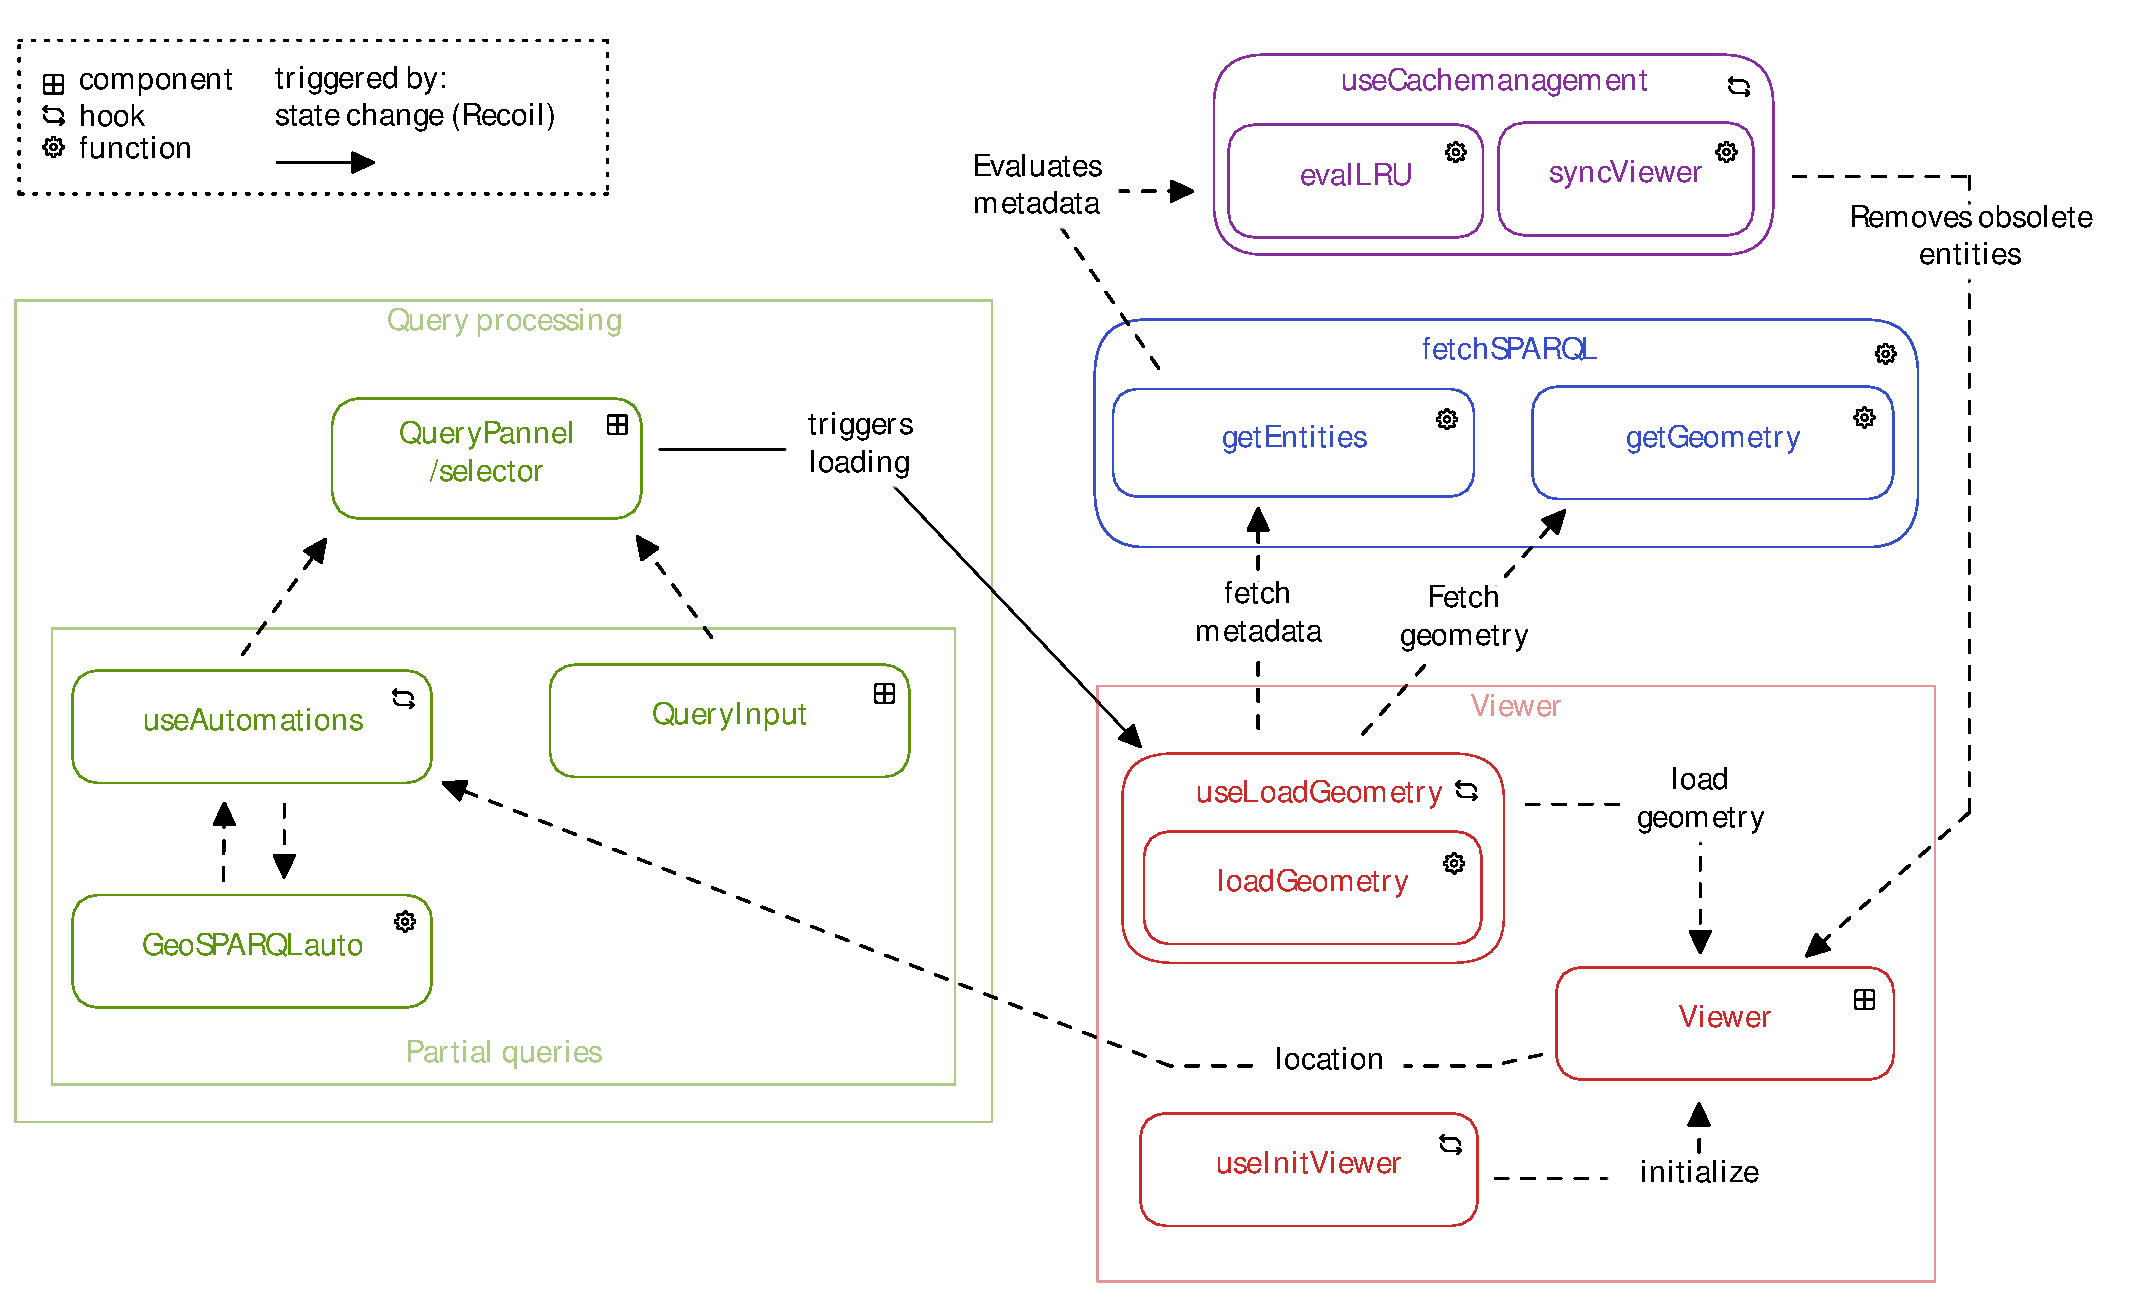
\includegraphics[width=\textwidth]{figures/pdf/interactions_prototype.pdf}
    \caption[Interactions prototype]{Conceptual diagram of the interactions between the modules within the prototype when using a dynamic query algorithm, such as GeoSPARQLauto, based on Figure \ref{fig:interactionModules}.}
    \label{fig:interactionPrototype}
\end{figure}

\section{Semantic visualisation} \label{sec:semanticVis}
\begin{listing}[H]
    \inputminted{ts}{dynamicQueries/colorize/type.ts}
    \caption[\acs{lru} entry type]{Type of the \ac{lru} entries, extendible to include additional metadata.}
    \label{lst:lruType}
\end{listing}

The cache management module is constructed in such a way that the \ac{lru} list stores metadata about the entities. Each entry in the cache management module is stored with a unique identifier, represented by its \ac{uri}. This identifier serves as the key for each entry. Correspondingly, the value of each entry is represented as a JavaScript object. As of the current state of the prototype, this object contains details such as the datatype and the format of the geometry. Therefore, this object can be extended to accommodate properties such as the non-geometrical ones described in Section \ref{sec:beyondGeometry}, as illustrated in its type description in Listing \ref{lst:lruType}.

\begin{listing}[H]
    \inputminted{json}{dynamicQueries/colorize/entry.json}
    \caption[LRU entry]{Example of an entry in the \ac{lru} list.}
    \label{lst:lruEntry}
\end{listing}

To illustrate this proposal, a triple containing color data was inserted into the database, with the query used shown in Listing \ref{lst:colorInsert}. The entry in Listing \ref{lst:lruEntry} displays the metadata stored in the \ac{lru} list for this entity. The color data is then applied to the geometry using the Xeokit \ac{api}. Since the latter does not allow color assignment during entity loading, the color is applied after the entity is loaded, within the syncViewer function (see Appendix \ref{sec:cache.ts}).

\begin{listing}[H]
    \inputminted{sparql}{dynamicQueries/colorize/insert.rq}
    \caption[Insert color data]{Insertion of color data into the database.}
    \label{lst:colorInsert}
\end{listing}

\section{Functionalities and Demonstration}
The main features of the prototype are available at:\\
\url{https://github.com/flol3622/Pre-culling_LDBIM#demo}\\
The following features were presented:

\begin{itemize}
    \item \textbf{Basic use case:} The basic use case is presented where the entire building is loaded with a maximum number of entities set to 20. The user can navigate through the building and entities are loaded on demand. The user can also change the maximum number of entities to be loaded at once.
    \item \textbf{Different sources and formats:} The prototype can load different sources and formats. A database of abstract shapes is selected which holds STL, OBJ and GLTF geometry files as literals or as links to external files on GitHub. (Section \ref{sec:viewerRequirements})
    \item \textbf{Semantic-driven filtering:} With the aid of semantics, the user can filter the entities to load in the viewer. This example filters the entities to only show the ones with \mintinline{sparql}|rdf:type prod:Window|.
    \item \textbf{Semantic-driven colorization:} Semantics associated with each entity can be used to colorize the entities in the viewer. This example colorizes the entities based on their \mintinline{sparql}|flupke:color| property which holds a color code. (Sections \ref{sec:visualSemantic}, \ref{sec:semanticVis})
    \item \textbf{In-query, OBJ-string analytics} A first culling algorithm is showcased where the \mintinline{sparql}|bot:Space| entities are filtered based on their OBJ definition, which is analyzed by the endpoint using a string operation. The cache management mechanism is also visualized as the viewer's scene does not exceed an entity count of 20. (Section \ref{sec:inQuery})
    \item \textbf{In situ, GeoSPARQL} This second culling algorithm uses GeoSPARQL functions. As the GeoSPARQL functions are limited to 2D space, the viewer hovering over a \mintinline{sparql}|bot:Space| triggers the loading of this last. (Section \ref{sec:inSituWKT})
\end{itemize}

The source code is available at: \url{https://github.com/flol3622/LDBIM-viewer}
